%%% Preamble
\documentclass[paper=a4, fontsize=11pt]{scrartcl}	% Article class of KOMA-script with 11pt font and a4 format
%\usepackage[T1]{fontenc}
\usepackage{fourier}
%\usepackage[sfdefault,light]{roboto}  %% Option 'sfdefault' only if the base font of the document is to be sans serif
\usepackage[T1]{fontenc}
\usepackage{float}

\usepackage[margin=1.2in]{geometry}
\usepackage{layout}

\usepackage[english]{babel}															% English language/hyphenation
\usepackage[protrusion=true,expansion=true]{microtype}				% Better typography
\usepackage{amsmath,amsfonts,amsthm}										% Math packages
\usepackage[pdftex]{graphicx}														% Enable pdflatex
\usepackage{url}

\usepackage[utf8] {inputenc}
\usepackage{setspace}
\onehalfspacing

%%% Custom sectioning (sectsty package)
\usepackage{sectsty}												% Custom sectioning (see below)
\allsectionsfont{\centering \normalfont\scshape}	% Change font of al section commands

\setlength{\footnotesep}{0.5cm}

%%% Custom headers/footers (fancyhdr package)
\usepackage{fancyhdr}
\pagestyle{fancyplain}
\fancyhead{}														% No page header
%\fancyfoot[L]{\small \emph{Dronecleaner}}		% You may remove/edit this line 
\fancyfoot[C]{}													% Empty
\fancyfoot[R]{\thepage}									% Pagenumbering
\renewcommand{\headrulewidth}{0pt}			% Remove header underlines
\renewcommand{\footrulewidth}{0pt}				% Remove footer underlines
\setlength{\headheight}{13.6pt}

%%% Equation and float numbering
\numberwithin{equation}{section}		% Equationnumbering: section.eq#
\numberwithin{figure}{section}			% Figurenumbering: section.fig#
\numberwithin{table}{section}				% Tablenumbering: section.tab#

%%% Maketitle metadata
\newcommand{\horrule}[1]{\rule{\linewidth}{#1}} 	% Horizontal rule

\title{
		%\vspace{-1in} 	
		\usefont{OT1}{bch}{b}{n}
		\normalfont \normalsize \textsc{INGENIØRHØJSKOLEN AARHUS UNIVERSITET} \\ [25pt]
		\horrule{0.5pt} \\[0.4cm]
		\huge ITBFIS - Håndbold applikation \\
		\horrule{2pt} \\[0.5cm]
}
\author{
		\normalfont 								\normalsize
        Darlow Kiruparajan 11605\\\normalsize Martin Due 11639\\\normalsize Andreas Andersen 11073\\\\[-3pt]		\normalsize
        15. januar 2015
}
\date{}

%%% Begin document
\begin{document}
\maketitle
\begin{figure}[ht!]
		\centering
		
\includegraphics[width=15mm]{images/handballl}
		\end{figure}


\newpage
\renewcommand{\figurename}{Figur}
\renewcommand\contentsname{Indholdsfortegnelse}
\tableofcontents

\newpage
\section*{Introduktion}
\addcontentsline{toc}{subsection}{Introduktion}
Til mindre håndbold stævner bliver der spillet mange kampe, men der bliver ikke ført statistik for de enkelte spillere. Derfor burde det være muligt for forældrene eller dommeren at lave en live statistik over hele håndbold kampen. Derved vil det være muligt for forældrene at se deres børns udvikling.\\\\
Dette kan løses vha. applikationer til mobileenheder, hvor der er muligt at oprette holdene og derefter lave en statistik. 

\subsection*{Problemformulering}
\addcontentsline{toc}{subsubsection}{Problemformulering}
I dette projekt vil vi ved hjælp af forskellige prototyper prøve at finde den bedste løsning til problemet nævnt i introduktionen. Dette skal gøres skal hjælp af usability tests, heuristisk evaluering og analyse af målt data fra forsøgpersoner.

\subsection*{Scenarie}
\addcontentsline{toc}{subsubsection}{Scenarie}
En bruger ankommer til en håndboldturnering, og ønsker at føre statistik for en kamp. Derfor opretter brugeren holdene for den kommende kamp således, at applikationen er klar til at lave en statistik.\\\\Kamp opsætning:
\begin{itemize}
\item Hold 1
	\begin{itemize}
	\item Holdnavn
	\item Spillernavne
	\item Antal spillere
	\item Målmands navn
	\end{itemize}
\item Hold 2
	\begin{itemize}
	\item Holdnavn
	\item Spillernavne
	\item Antal spillere
	\item Målmands navn\\
	\end{itemize}
\end{itemize}
Når opsætning  er fuldført, kan kampen startes og brugeren kan begynde at lave statistik over kampen.\\\\
Liste over mulige begivenheder:
\begin{itemize}
	\item Hold X, Spiller X – Score
	\item Hold X, Spiller X – Saved
	\item Hold X, Spiller X – Missed
	\item Hold X, Spiller X – Blocked\\
\end{itemize}
Når kampen er afsluttet, kan brugeren få vist statistik over hele kampen.\\\\Da brugergruppen er forældre, er det vigtig, at applikationen har en nem brugergrænsefalde (usability). Til at løse usability, kan man benytte design konventioner, hvilket vil give brugeren et mere ensartet design, som ligner andre applikationer. For at kunne se user experience issues, er det muligt at lave nogle forskellige tests af applikationerne. Derved er det muligt at undersøge usability for applikationerne og for brugerne. 

   
   


\newpage
\section*{Personas}
\addcontentsline{toc}{subsection}{Personas}
\textbf{Kamilla:}
\addcontentsline{toc}{subsubsection}{Kamilla}
\begin{itemize}
\item 	Baggrund
	\begin{itemize}
	\item 36 år
	\item Gift med Anders på 37.
	\item Mor til 2 (Jesper på 9. og Ginnie på 6.)
	\item Vil gerne involvere sig i sine børn.
	\item Bruger teknologi i sin dagligdag
  	\end{itemize}	
\item Motivation
	\begin{itemize}
	\item Være den ``bedste" mor i klassen.
	\item Hjælpe sine børn med at blive de bedste til alt hvad de gør.
	\item Fremstå som velovervejet for omverdenen.
	\end{itemize}
\item Frustrationer
	\begin{itemize}
	\item Inkompetence ved andre.
	\item Når der ikke er tid nok.
	\item At lave valg/udtalelser uden tilstrækkelig viden.
	\end{itemize}
\item Persona
	\begin{itemize}
	\item Kamilla er en rigtig husmor, som vil være sikker på at famillien har det godt, hun sørger for at maden er klar når Anders kommer hjem fra arbejde.
	\item Hun sikre sig at Jesper og Ginnie bliver hentet i ordentlig tid fra skole, så de kan komme til deres fritids aktiviteter.
	\item Kamilla tager ofte til håndbold turnering for at se sin søn Jesper spille for håndboldklubben Århus Håndbold Klub(ÅHK).
	\item Jesper spiller venstre Bak, og er meget motiveret for at blive bedre, og være den bedste spiller på holdet, hvilket Kamilla gerne vil støtte ham i.
	\end{itemize}
\end {itemize}

\newpage
\textbf{Teis:}
\addcontentsline{toc}{subsubsection}{Teis}
\begin{itemize}
\item 	Baggrund
	\begin{itemize}
	\item 52 år.
	\item Fraskilt.
	\item Gammel håndbold spiller.
  	\end{itemize}	
\item Motivation
	\begin{itemize}
	\item Hjælpe den unge generation til at blive gode til håndbold.
	\item blive bedre til at se på statistik når han ser TV.
	\end{itemize}
\item Frustrationer
	\begin{itemize}
	\item ex-konens konstante klagen over at han bruger for meget tid i klubben.
	\end{itemize}
\item Persona
	\begin{itemize}
	\item Teis har været frivillig i den lokale håndbold klub i lang tid og begyndte at bruge mere tid efter at hans kone gik fra ham.
	\item Han sidder ofte ved dommer bordet og registrere mål/udvisninger ol. i løbet af håndboldkampe.
	\item Teis vil gerne være med til at gøre Håndbold mere attraktivt for folk at følge, og er derfor begyndt at involvere sig i Dansk håndboldforbunds arbejde, og især ved at give input til hvad der skal ligge på deres hjemmeside.
	\end{itemize}
\end {itemize}


\newpage
\section*{Low-fidelity prototyper}
\addcontentsline{toc}{subsection}{Low-fidelity prototyper}
\subsection*{Udvikling af prototyper}
\addcontentsline{toc}{subsubsection}{Udvikling af prototyper}
Da vi allerede havde en ide om hvad vores produkt skulle kunne, startede vi vores udvikling af prototype ved hjælp af "scenario analysis" samt "task analysis", da vi havde et begreb for hvad vi ville kunne med vores prototype, begyndte vi at lave en "mundtlig brainstorm", for at finde frem til mulige løsninger. Dette resulterede i begge vores prototyper. Vi lavede efterfølgende "think-aloud" tests for at hører hvad der kunne gøres bedre eller hvad der var godt ved vores prototyper.

\subsection*{Test af prototyperne}
\addcontentsline{toc}{subsubsection}{Test af prototyperne}
Der var 2 personer til at lave Think-aloud test af Low-Fi prototyperne. De var begge førstegangs brugere. Da ingen af dem havde større kendskab til håndbold, var vi nød til at beskrive hvad applikationens hensigt var, samt at give dem en kort introduktion til domænet.\\\\ \textbf{Prototype 1, baggrundstanker:}
Ideen med denne prototype, var at den skulle benyttes på en touch-skærm, med en størrelse på ca 7"-10".(tablet-size)
Det var hensigten at bringe så meget af domænet ned i applikationen. og altså tegne banen op, og give brugeren mulighed for at sætte spilleren på sin plads på banen, i stedet for at vælge positionen fra de mulige (fløj, bak, center ol.)\\\\ \textbf{Beskrivelse af Prototypen:} Denne prototype blev udarbejdet ved brug af post-its og transparente A4-sider. Vi brugte hvid A4 papir, som baggrund. der var et ark papir, for hvert layout af baggrund,knapper og informationer.
Vi brugte transparent A4, til at symbolisere pop-up skærme, så det var tydeligt for test-personen at han ikke blev fjernet fra den foregående side.
og vi brugte post-its til de genstande, der skulle kunne flyttes rundt på.\\\\\textbf{Resultat af think-aloud test:} Begge test personer syntes at denne prototype var meget intuitiv. og det var kun en enkelt gang at den ene test person var i tvivl om hvordan en given task skulle løses. og de var derudover meget tilfredse over applikationen.\\\\ \textbf{Prototype 2, baggrundstanker:} Denne prototype, var blev udviklet efter princippet "det bedste produkt, er det du har ved hånden" (ok, den fandt jeg selv på :P) Men det ændre ikke på at det var grunden til at vi ville teste om der ville være større tilfredshed med en mobilapplikation.
Denne prototype bygger på mange af de samme principper som den prototype der blev lavet til tablet. men da skærmen er meget mindre, valgte vi at fjerne "baggrunds billedet" og i stedet benytte tekst og knapper.\\\\ \textbf{Beskrivelse af prototypen:} for at lave en Low-Fi prototype klippede vi nogle stykker papir ud, på størrelse med en smartphone skærm, derefter tegnede vi de forskellige sider man kunne navigere rundt imellem. mindre stykker papir representerede "pop-ups" så man ikke troede at man skiftede billede. \textbf{Resultat af Think-aloud test:} Generelt syntes begge test personer at det hele var "for småt" (det mente vi dog skyldtes dårlig håndskrift). derudover havde denne prototype langt større problem, fordi den stillede størrer krav til brugerens domæne kendskab. og vi ente derfor med at være nød til at hjælpe dem med at udfylde disse, på denne prototype.


\section*{Hi-fidelity prototyper}
\addcontentsline{toc}{subsection}{Hi-fidelity prototyper}
Hi-fidelity prototyperne valgte vi at lave på to forskellige måder. Den ene kaldet \emph{Prototype 1} ved hjælp af HTML, Javascript og CSS og den anden kaldet \emph{Prototype 2} som en Android applikation, der kører på en mobiltelefon. Med disse teknologier kunne vi styre præcist hvordan prototyperne skulle fungere, og det var forholdsvist hurtigt at lave forbedringer eller rettelser til hver især. Dog var det hurtigst at lave rettelser til prototype 1. Med disse teknologier kunne prototyperne testes på computer, tablet og mobiltelefon for at emulere hvordan vores scenarie for en håndboldkamp hang sammen. Grundidéen var at en person trackede en håndbold kamp, så derfor ville vedkommende højst sandsynligt sidde med et bærbart device ved sin sinde.\\\\Prototyperne gør det muligt at gennemgå en række tasks i et flow, der er bestemt på forhånd. For at beskrive flowet er det opstillet i rækkefølge nedenfor:
\begin{enumerate}
\item Indtast spillernavne for begge hold. (Task 1)
\item Drag and drop spillertrøje ind på de korrekte pladser. (Task 2)
\item Start kampen og godkend dermed at positionerne er korrekte. (Task 2)
\item Indtast de forskellige skudforsøg der opstår under kampen for hver spiller. (Task 3)
\item Afslut kampen når sidste fløjt går. (Task 3)
\item Se spillerstatistik og holdstatistik når kampen er slut. (Task 4)\\\\
\end{enumerate} 

\newpage
\subsection*{Visning af prototypen}
\addcontentsline{toc}{subsubsection}{Visning af prototypen}
For at imødekomme de forskellige designregler vi har haft om i kurset som f.eks. gestalt teori har vi arbejdet det ind i prototyperne. I gestalt er der regler om:
\begin{itemize}
\item Reglen om nærhed
\item Reglen om ensartethed
\item Reglen om lukkethed
\item Reglen om symbolik\\
\end{itemize}

\begin{figure}[ht!]
\centering
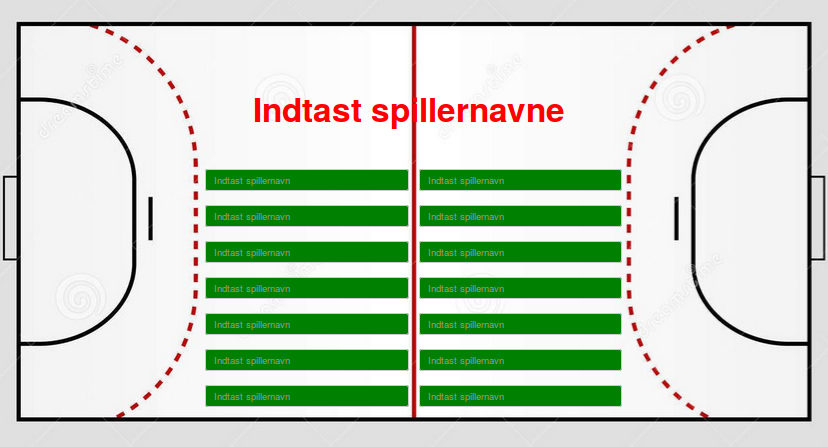
\includegraphics[width=150mm]{images/begin}
\caption{Prototype 1}
\end{figure}
På prototype 1 ses det hvordan vi har grupperet inputfelterne, så brugeren ved hvad der skal ske. De er for det første delt op i to grupper, så man let regner ud hvilke grupper der hører til hvilket hold. Alle felterne er ens, så man véd at det samme skal gøres med hvert felt. På grund af at vi har anvendt Bootstrap til vores CSS er inputfelterne lukket inde i en boks samtidig med at de med gestalt reglen om symbolik ligner noget brugeren har set før på internettet.\\\\

\newpage
På prototype 2 ses det ligeledes hvordan felterne er grupperet således de opfylder gestalt reglerne om nærhed, ensarthedhed samt symbolik, da de ligner andre input felter i Android applikationer. Som standard er felterne ikke lukkede af, men da skærmen er så lille ved brugeren at de hører sammen.
\begin{figure}[ht!]
\centering
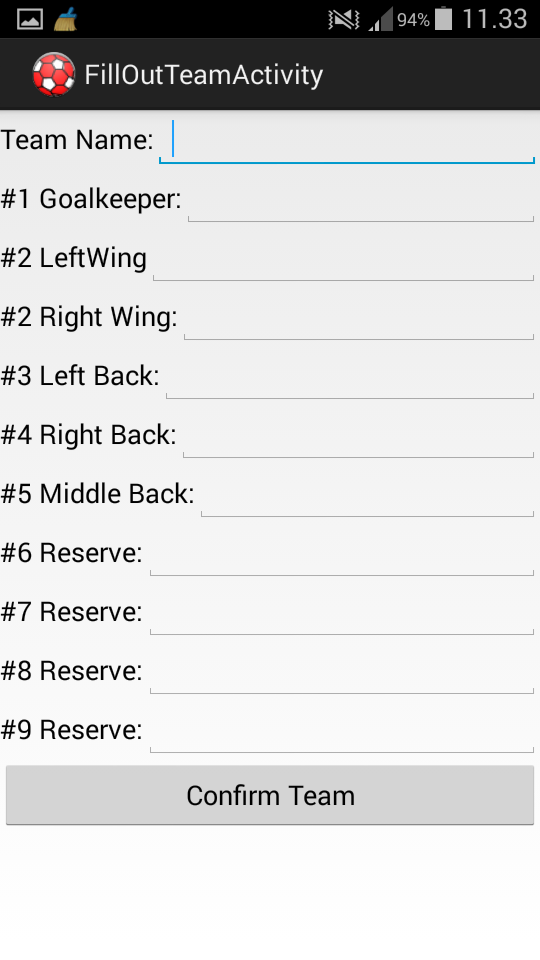
\includegraphics[width=50mm]{images/prototype2}
\caption{Prototype 2}
\end{figure}

\newpage
\subsection*{Peer review outcome}
\addcontentsline{toc}{subsubsection}{Peer review outcome}
Efter udvikling af prototyperne brugte vi andre personer til at teste dem for os. Dette blev gjort først for at se om brugere overhovedet kunne komme sikkert igennem prototyperne for at lave en binær statistik over dette. Det viste sig hurtigt at de brugere, der hjalp os, var ret kendte på disse typer af applikationer, hvilket nok skyldes de teknologier, der bruges og klassen var fuld af ingeniørstuderende.\\\\Eksempler på hvad vi fik ud af peer reviews:
\begin{itemize}
\item Det var farligt at komme til at dobbeltklikke på knapper, da man kom for langt i flowet.
\item Man kunne ikke gå baglæns i flowet.
\item Det er ikke sikkert der er præcis så mange personer på et hold.
\item Man kunne ikke se antal mål under kampen.
\item Screen scrolling er irriterende for brugeren.\\\\
\end{itemize} 

Den binære statistik viser hvordan brugerne klarede task 1 på prototyperne i forhold til hinanden.
\begin{figure}[ht!]
\centering
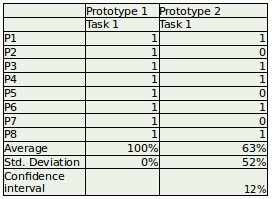
\includegraphics[width=100mm]{images/binary}
\caption{Binær data}
\end{figure}
Det ses at på prototype 1 kom alle igennem task 1, hvor på prototype 2 på mobiltelefonen kom alle ikke igennem. Derfor opfyldte prototype 1 altså formålet langt bedre. Desuden kunne vi bruge de forskellige rettelser brugerne kom med til at forbedre prototypen, feks. ved at flytte knapper rundt, så man ikke dobbeltklikkede på dem.\\\\

\subsection*{Think aloud test}
\addcontentsline{toc}{subsubsection}{Think aloud test}
Da interaction design kan virke som en let forståelig opgave, er det vidt forskelligt hvordan mennesker opfatter brugergrænseflader i forhold til hinanden. Defor lavede vi en think aloud test på prototype 1 for at se hvordan en uvedkommende person tænkte om prototypen. Her fandt vi blandt andet ud af at han genkendte designet fra andre lignende applikationer, men at han gerne ville se hvor mange mål han havde indtastet f.eks. i task 3.\\\\ 

\subsection*{Metrics and statistics}
\addcontentsline{toc}{subsubsection}{Metrics and statistics}
For at måle de to forskellige prototyper fra hinanden lavede vi statistik over time on task. 
\begin{figure}[ht!]
\centering
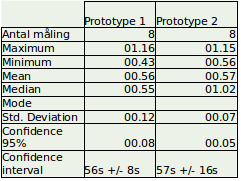
\includegraphics[width=100mm]{images/timeontask}
\caption{Time on task}
\end{figure}
Ved måling af dette var der umiddelbart ikke stor forskel på de forskellige prototyper, men som man kan se på statistikken er der forholdsvis stor afstand mellem max og min på prototype 1, hvilket gav en indikation af, at man måske kunne træne brugeren til at blive bedre i prototypen. Det gav anledning til at lave en learnability statistik over prototype 1.\\\\

\newpage
\begin{figure}[ht!]
\centering
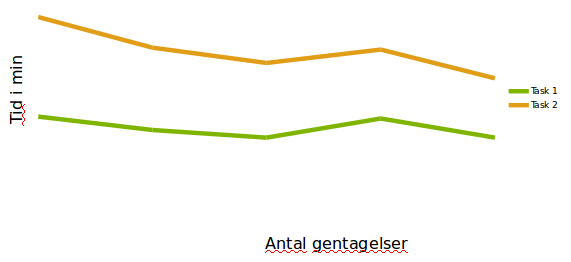
\includegraphics[width=100mm]{images/learnability}
\caption{Learnability curve}
\end{figure}
På kurven Learnability kurven ses det hvordan en bruger langsomt bliver hurtigere og hurtigere til at komme gennem prototypen. Og da det er en applikation, som brugeren gerne må bruge tid på inden en eventuel håndboldkamp er dette rigtig godt. 





\newpage
\section*{Konklusion}
\addcontentsline{toc}{subsection}{Konklusion}
Vi valgte ikke at bruge standardprojektet, men i stedet lave en applikation der handlede om håndboldstatistik. For at gøre det mere realistik oprettede vi to forskellige personaer, som projektet kunne være relevant for, og det gav os en retning at udviklede efter.\\\\I løbet af dette projekt har vi arbejdet med tre forskellige prototyper. Efter de første usability tests i projektet fandt vi hurtigt ud af, at prototype 1 nok var den bedste at gå efter, nummer 2 var interessant at følge og nummer 3 skulle smides væk efter samtale med de første testpersoner. Det viste sig også i de efterfølgende usability tests af de to prototyper at prototype 1 var den bedste. Både i binary success rate, time on task og satisfaction var prototype 1 den førende. Derfor i videre udvikling af projektet ville vi fokusere på prototype 1.\\\\Vi har lært at arbejde med forskellige metrics, og analyseret den data vi har fået ud af vores forskellige tests. Blandt andet kunne vi stille task success rate op for de to prototyper i forhold til hinanden, og se at prototype 1 umiddelbart var den bedre. Da time on task målingerne lå så tæt på hinanden overlappede deres confidence interval, og det var derfor ikke muligt at fastslå om den ene prototype var bedre end den anden, men i de pågældende testmålinger havde prototype 1 stadig de bedste resultater.\\\\Udover dette har vi lavet en learnability curve for at se én brugers udvikling med gentagne gennemgange af testscenariet på prototype 1. 

%%% End document
\end{document}